%%%%%%%%%%%%
\documentclass[11pt]{article}
\usepackage{latexsym}
\usepackage{amsmath}
\usepackage{graphicx}
\usepackage{amssymb}
\usepackage{natbib}
\usepackage{textcomp}
\renewcommand{\thesection}{\hspace*{-1.0em}}
\renewcommand{\thesubsection}{\arabic{subsection}}
\usepackage{booktabs}

\DeclareGraphicsExtensions{.pdf,.png,.jpg}
\usepackage[top=1in, bottom=1in, left=1in, right=1in]{geometry}
\usepackage{pgfplots}
\pgfplotsset{width=7cm,compat=1.8}
\parindent0pt
\usepgfplotslibrary{statistics}
\parskip\bigskipamount

\newtheorem{thm}{Theorem}
\newtheorem{cor}{Corollary}
\newtheorem{exa}{Example}
\newtheorem{ass}{Assumption}
\newtheorem{pro}{Proposition}
\newtheorem{defn}{Definitions}
\newtheorem{lem}{Lemma}
\newtheorem{pf}{proof}
\newtheorem{remark}{Remark}

\title{2018 INFORMS O.R. {\&} Analytics Student Team Competition}

\author{\textbf{Entry Number: [}2018ORASTC252]
}

\date{}

\begin{document}
	
	\maketitle
	
	%\centerline{\textbf{2018 INFORMS O.R. {\&} Analytics Student Team Competition -- ENTRY FORM}}
	
	\baselineskip16pt plus 1pt minus 1pt
	
	
	%\textbf{Entry Number: [}2018ORASTC252]
	
	\section*{Executive Summary (not to exceed 2 pages)}
	%\textbf{Executive Summary (not to exceed 2 pages)}\\*
	
	
	\section*{Team Makeup {\&} Process}
	
	Our team consists of three undergraduate students whose major is in industrial and management engineering and an advisor whose research field is Operation Research. We worked together on a variety of projects, including data mining projects and optimization modeling projects during the classes in college. Finally, The three of us enjoy to challenge and we enter 2018 INFORMS O.R. {\&} Analytics Student Team Competition as a final challenge before graduating from college. 
	\begin{figure}[h] 
		\begin{center}
			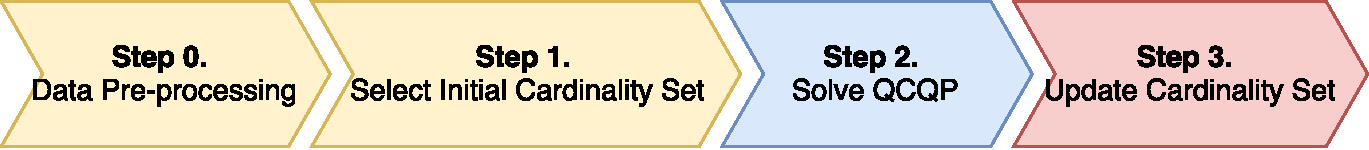
\includegraphics[width=0.7\textwidth]{process2}
			\caption{The process of the project} \label{fig:process}
		\end{center}
	\end{figure}
	One of us has patented a great algorithm to solve the 'Chinese postman problem’, and applied it to the problems of the real world and developed the mobile application and started the business. He is a development worker at the start-up company. He works on solving the portfolio optimization through the formulation based on his experience of dealing with various optimization tools. Another team member has experience in refining and analyzing real data in various companies, and is especially interested in deep learning,  which is the most recent issue. This personal background could be the idea for the project and develop a deep learning based algorithm which makes our algorithm be the best. Our algorithm includes various technical contents such as parallel processing to derive the solution widely. Our last team member contributes to make our heuristic algorithm faster and more powerful with his experience in developing a system. The Advisor give guidance on the algorithm presented through the weekly meetings, 교수님의...엄청난 지도... Above all, the teamwork is the most important factor in developing the best algorithms by maximizing each experience and background. 
	From understanding the problem to developing the best algorithm, all process was a series of challenges. Our first challenge was to understand and analyze the business model correctly. The actual data given is very different from what is commonly known, but we tried to solve by analyzing actual stock data as well as related papers through seminar every week. Our second challenge was to develop a methodology that fits the problem situation through a deep understanding of the problem. In particular, the number of stocks to be considered may be large in the real world, so we devised a method of separating the process of selecting the set of assets to invest and determining the weight of the asset so as not to be sensitive according to the problem size.
	We keep challenging ourselves, and we grow up through trial and error during the four months. As a result, we develop an organic algorithm that includes the process from step1 to step3. 
	
	
	\section*{Framing the Problem}
	Portfolio optimization is finding the optimal proportion of each asset in an investor’s portfolio. In the problem given, the investors construct an investment portfolio to minimize risk. The investment portfolio is also required to satisfy not only the well-known Markowitz formulation constraints, but also the extension constraints that reflect the actual situation. First, We take a look at the meaning of each constraints in the formulation presented and give a suggestion on how to handle the constraints.
	The parameters and decision variables are defined as follows:
	\begin{description}
		\item[$N$]: set of assets
		\item[$w^{bench}_i$]: weight of benchmark of asset $i \in N$
		\item[$\Omega \in \mathcal{R}^{|N|\times |N|}$]: return covariance matrix for all assets in the universe, which contains the relationships between each pair of historical return series. $\Omega$ is a symmetric matrix where the diagonal elements are the variances of the asset returns, the off-diagonal elements are covariances.
		\item[$\alpha_i$]: Expected return score of asset $i \in N$, higher values are expected to have higher future returns.
		\item[$\beta_i$]: measure of return sensitivity relative to the equity market return as a whole of asset $i \in N$ 
		\item[$S$]: set of sectors
		\item[$N_s$]: set of assets of sector $s \in S$
		\item[$K$]: set of MCAPQ (Market Cap Quintile)
		\item[$N_k$]: set of assets of MCAPQ $k \in K$
		\item[$w_i$]: decision variable, weight of asset $i \in N$
		\item[$d_i$]: decision variable, difference between weight and the benchmark of asset $i \in N$
	\end{description}
	
	
	For a given asset $i \in N$, $d_i$ is defined as
	\begin{align}
	d_i = w_i - w^{bench}_i. \label{eq:P:activeweight}
	\end{align}
	
	Then, the mathematical formulation for the portfolio selection problem is stated as:
	\begin{align}
	\text{(P)} \quad \min~ & d^T \Omega d - \lambda d^T \alpha \label{eq:P:obj}\\
	\text{s.t. } 
	& w_i \ge 0, & \forall i \in N, \label{eq:P:nonn}\\
	& \sum_{i \in N} w_i = 1, \label{eq:P:sum}\\
	& -0.05 \le d_i \le 0.05, & \forall i \in N, \label{eq:P:d}\\
	& -0.1 \le \sum_{i \in N_s} d_i \le 0.1, & \forall s \in S, \label{eq:P:sector}\\
	& -0.1 \le \sum_{i \in N_k} d_i \le 0.1, & \forall k \in K, \label{eq:P:MCAPQ}\\
	& -0.1 \le \sum_{i \in N} \beta_i d_i \le 0.1, \label{eq:P:beta}\\
	& 50 \le card(w_i \neq 0) \le 70, \label{eq:P:card}\\
	& 0.6 \le 1 - \sum_{i \in N} \min\{w_i, w^{bench}_i \} \le 1, \label{eq:P:AS}\\
	& 0.05 \le \sqrt{d^T \Omega d} \le 0.1, \label{eq:P:TE}
	\end{align}
	where $card(w_i \neq 0)$ represents the number of weights that are greater than a given threshold 0.001. The objective function \eqref{eq:P:obj} minimizes the sum of total risk ($d^T \Omega d$) and the negative of expected return ($d^T \alpha$), weighted by parameter $\lambda$ that controls the trade-off between the risk and expected return. Constraints \eqref{eq:P:nonn} - \eqref{eq:P:beta} are linear, each of which represents a specific business requirement. 
	Constraints \eqref{eq:P:d} ensures that $[-0.05, 0.05]$, and it can be expressed as : $w^{bench}_i-0.05 \le w_i \le w^{bench}_i+0.05$ for all $i \in N$ . When the lower bound of the weight is bigger than 0.001, it should be included in the set of assets to invest.  For each set of sector $s \in S$ and MCAPQ $k \in K$, the sum of the active share must be in the range $[-0.1, 0.1]$. 
	Not only the number of assets included in each sector and MCAPQ is different, but also the sum of bench weights is different. (Additional Analysis)  Constraint \eqref{eq:P:card} restricts the number of positive weights, which make the problem non-convex because of the non-convex function $card(w_i \neq 0)$. Nonetheless, constraint \eqref{eq:P:card} can be linearized by introducing some binary decision variables as shown in the following proposition.
	\begin{pro} \label{pro:AS}
		Constraint \eqref{eq:P:card} can be replaced by the following set of constraints:
		\begin{align*}
		&y_i \ge w_i, & \forall i \in N, \\
		&y_i \le w_i + 0.999, & \forall i \in N,\\
		&50 \le \sum_{i \in N} y_i \le 70, \\
		&y_i \in \{0,1\}, & \forall i \in N.
		\end{align*}
	\end{pro}
	Constraint \eqref{eq:P:AS} restricts the active share of the portfolio between 0.6 and 1. Because $w_i \ge 0$ and $w^{bench}_i \ge 0$ for any $i \in N$, the constraint $1 - \sum_{i \in N} \min\{w_i, w^{bench}_i \} \le 1$ is redundant, which results in the following proposition.
	\begin{pro}\label{pro:TE}
		Constraint \eqref{eq:P:AS} can be replaced by the following set of constraints:
		\begin{align*}
		& 0.6 \le 1 -  \sum_{i \in N} v_i,\\
		& w_i - z_i \le v_i \le w_i, & \forall i \in N,\\
		& w^{bench}_i - 1 + z_i \le v_i \le w^{bench}_i, & \forall i \in N,\\
		& z_i \in \{0,1\}, & \forall i \in N.
		\end{align*}
	\end{pro}
	
	Constraint \eqref{eq:P:TE} ensures the tracking error (TE) to be in the given range $[0.05,0.1]$. In general, a higher TE means the portfolio would be more volatile, while a lower TE indicates the portfolio closely would follow the benchmarks. Constraint \eqref{eq:P:TE} consists of two inequalities: $0.05 \le \sqrt{d^T \Omega d}$ and $\sqrt{d^T \Omega d} \le 0.1$, where the latter is a convex constraint. The former inequality, however, is non-convex. 
	
   Tracking error and active share are measures of how different the investment portfolio is from the benchmark, a composite indicator derived from several accumulated criteria. In both investment portfolios, the absolute difference between portfolio weight and bench weight is the same, but let's consider the case where portfolio weight is biased toward one or two assets. Since the two have the same absolute value of the active weight, the active share is the same. Likewise, active share ignores diversification, so 
   
	
	
	By using Proposition \ref{pro:AS} and \ref{pro:TE}, we can formulate a mixed integer non-linear programming (MINLP) problem. There are several solvers for obtaining global optimal solutions of the MINLP problems such as BARON (ref.), Couenne (ref.), and Bonmin (ref.). Those solvers typically incorporate outer approximation/generalized Bender's decomposition into branch-and-bound framework. Existence of many binary decision variables and non-convex constraints, however, makes solving of the formulation directly using the off-the-shelf solvers intractable. 
	
	
	
	
	
	\section*{Data}
	The data from Principal consists of 3 parts which are timeseries data, riskmodels data, and result template data. Timeseries data and riskmodels data contain the parameters for portfolio optimization, and result template data contains indicators for evaluating solution quality after deriving the final solutions. The details of each data for the portfolio optimization problem are listed as follows. 
	
	\begin{itemize}
		\item \textbf{Time Series Data} : It contains the parameter values needed to construct the formulation for each period. At this time, not only does it contain unique information of assets like SEDOL or Sector that do not change, but it also includes Alpha score$\alpha$, Beta$\beta$, Bench Weight$w_{\text{bench}}$, and MCAPQ, which describe the characteristics of the asset at each period.
		\item \textbf{Riskmodels Data} : The risk is composed of diagonal elements representing the risk of each asset and off-diagonal elements representing the risk between the two assets. It is important that not only the variances of the return values of the diagonal elements are minimized, but also the large assets of the omega between the two assets are not selected together.
		\item \textbf{Result Template Data} : It contains 4 weekly forward returns, and is used when calculating portfolio performance. 
	\end{itemize}
	
	
	\subsection{Data Pre-processing and Rescailing}
	
	There are some difficulties in applying the data given from Principal directly to the model. Therefore, we present the following data preprocessing process. To make the data composed of three parts more flexible, a process of data preprocessing formed dataframe using the Pandas Library (http://pandas.pydata.org) in Python. In particular, as rebalancing is carried out, it is configured to extract not all time series data, but only the data needed for the iteration. The parameters used in model were extracted from data frames formed for each period, when each parameter (Alpha Score($\alpha$), Beta($\beta$),4 Weekly Returns ($r$), etc) was set with the 'SEDOL' index as the key value. This dictionary data type is proper to consider a list of assets that may change every period. The parameter Omega ($ \Omega $) is specified as the covariance matrix for a given data. In this case, the index in the columns and rows are 'SEDOL', the key value of the time series dictionary derived from the above, and are constructed in the form of full matrix. Taking the first period data as an example, we realize that the range of $\Omega$ is (from -0.024 to 0.616) and the range of $\alpha$ is (from -2.1e-05 to 1.9e-05). Especially, The $\Omega$ is less influential because it is considered with a very small value of active weight. Because the value of data is small, it may cause a calculation error due to the limit value of Python, and the value may be ignored in optimization tool, CPLEX. Therefore, we prevent several problems that can occur by multiplying $\alpha$ and $\Omega$ to 10000. By multiplying $\alpha$ and $\Omega$ to 10000, we multiply both sides of the Constraints(11) equally by 10000. 
	
	
	\subsection{The Analysis of the Data}
	% MCAPQ 와 SECTOR별 Weight의 범위 (결과?와 연관지어서)
	% Active Share과 Tracking Error의 관계 (데이터 기반)
	% 추가 historical 데이터 확보 및 분석 --> omega 도출 결과 corelation이 낮음 => 이유 간단히 분석?
	
	
	\section*{Methodology Approach {\&} Model Building}
	\setcounter{subsection}{0}
	
	
	\subsection{Preliminary Tests}
	
	% CPLEX를 가지고 QCQP 풀었을 경우 (1) Linearlize (2) Handling non-convex constraints -> Bisearch Approach (3)간단한 실험 (4)실험결과 분석 (문제를 어렵게 만드는 제약조건 , cardinality 제약식)
	In order to assert the difficulty of the problem (P), we conducted a test using the following simplified formulation:
	\begin{align*}
	\text{(P1)} \quad \min~ &\eqref{eq:P:obj}\\
	\text{s.t. } 
	& \eqref{eq:P:activeweight}, \eqref{eq:P:nonn} - \eqref{eq:P:beta}, \notag\\
	& y_i \geq w_i, & \forall i \in N, \tag{9-1*}\\
	& y_i \leq w_i + 0.999, & \forall i \in N, \tag{9-2*}\\
	& 50 \leq \sum_{i \in N} y_i \leq 70 \tag{9-3*}\\
	& y_i \in \{0,1\}, & \forall i \in N, \tag{9-4*}\\
	&  d^T \Omega  d \  \leq 0.01. & \tag{11*}
	\end{align*} 
	Constraints (9-1*)-(9-4*) are due to Proposition \ref{pro:AS}. Constraint (11*) is obtained by squaring both sides of constraint \eqref{eq:P:TE}. Note that the problem (P1) is a relaxation of (P) due to lack of constraint \eqref{eq:P:AS} and non-convex part of constraint \eqref{eq:P:TE}. The problem (P1) is a mixed integer quadratic constrained quadratic programming (MIQCQP) problem that can be solved by off-the-shelf solvers such as CPLEX (ref.). The decision variables $y_i$ is 1 if asset $i \in N$ is selected (i.e., $w_i \ge 0.001$). We solved (P1) for the time period of January 2007 with CPLEX 12.6 on a MacPro machine with Intel Xeon 3.5GHz CPU. 
	
	\begin{table}[]
		\centering
		\footnotesize 
		\caption{The results of solving (P1) by CPLEX}
		\label{tab:pre}
		\begin{tabular}{cccccc}
			\toprule
			\textbf{B\&B time (sec)} & \textbf{\# of feasible} & \textbf{GAP(\%)} & \textbf{Tracking Error} & \textbf{Active Share} & \textbf{Violated Constraints} \\
			\midrule
			\textbf{30} & 0 & - & - & - & -  \\
			\textbf{60} & 0 & - & - & - & -  \\
			\textbf{90} & 2 & 100.3\% & {\color[HTML]{CB0000} 0.0018} & 0.72 & (11) TE \\
			\textbf{120} & 2 & 100.3\% & {\color[HTML]{CB0000} 0.0012} & 0.64 & (11) TE \\
			\textbf{150} & 2 & 100.3\% & {\color[HTML]{CB0000} 0.0018} & 0.72 & (11) TE \\
			\textbf{180} & 8 & 100.6\% & {\color[HTML]{CB0000} 0.0004} & {\color[HTML]{CB0000} 0.50} & (10) AS, (11) TE  \\ 
			\bottomrule
		\end{tabular}
	\end{table}
	
	Table \ref{tab:pre} shows the number of integer feasible solutions found by branch and bound for a given time. The column GAP represents the difference (\%) from the best low bound, which is given as $\frac{\text{obj. value of best integer solution-best lower bound}}{\text{obj. value of best integer solution}} \times 100$. Large GAPs shown in the table imply that the problem (P1) is pretty hard to solve, even it is significantly relaxed from the original problem (P). Non of the test cases could find an optimal solution within 3 minutes, which means that solving the formulations (P1) or (P) directly using off-the-shelf solvers is hopeless. 
	
	The calculated values of AS and TE from the best integer solutions are also shown in the table. We found that among constraints for the AS and TE, the constraint for the TE ($0.05 \le \sqrt{d^T \Omega d}$) is more prone to violate, which is understandable by noting that the TE is supposed to be minimized from the objective function. Based on the results of the preliminary experiments, the following observations were derived.
	\begin{description}
		\item \textbf{(O1)} Due the existence of many binary decision variables, it is very hard to solve problem (P) as it is.
		\item \textbf{(O2)} Once the binary decision variables were fixed, solving (P1) is easy (e.g., less than a second).
		\item \textbf{(O3)} The constraints for the TE and AS must be addressed separately to ensure feasibility.
		\item \textbf{(O4)} In particular, TE values of the portfolios must be increased to satisfy constraint \eqref{eq:P:TE}.
	\end{description}
	
	Motivated by the above observations, we propose a three-phase heuristic approach. The first phase determines a set of assets to invest. Pre-determination of the set of assets enables us to eliminate most of binary decision variables from the problem (P1). The second phase involves finding of feasible solutions under the given set of assets. The basic idea for this is to solve (P1) after fixing the binary decision variables $y_i$ according to the given set of assets. When the solution if infeasible to either \eqref{eq:P:AS} or \eqref{eq:P:TE}, we add some constraints to the formulation (P1) to make the portfolio have higher TE value. The last phase improves the feasible portfolio by repeatedly updating the pre-determined set of assets. In the following sections, we explain each phase in details.
	
	\subsection{Phase 1: Selection of Initial Set of Assets to Invest}
	
	This phase needs to select an initial set of assets to invest. Ideally, selection of assets to invest must be able to consider all constraints of (P) and the objective function. Our computational experiments discourage any mathematical programming based approach for this purpose, because of too many binary decision variables. We propose a generative adversarial network (GAN) based approach. Before presenting the detailed algorithm developed, we first give a rather brief introduction on the GAN.
	
	
	\subsubsection{Generative adversarial networks (GANs)}
	
	A GAN is a variant of deep neural net (DNN) architectures comprised of two networks (ref.). One neural network, called \textbf{Generator (G)}, generates new data instances, while the other, \textbf{Discriminator (D)}, decides whether each instance of data is real (real images) or fake (generated by G). Both neural networks learn to alternate with each other. The G trains to generate data similar to real data in order to deceive D, and the D trains to distinguish real data from fake data generated by G. 
	\begin{figure}[h] 
		\begin{center}
			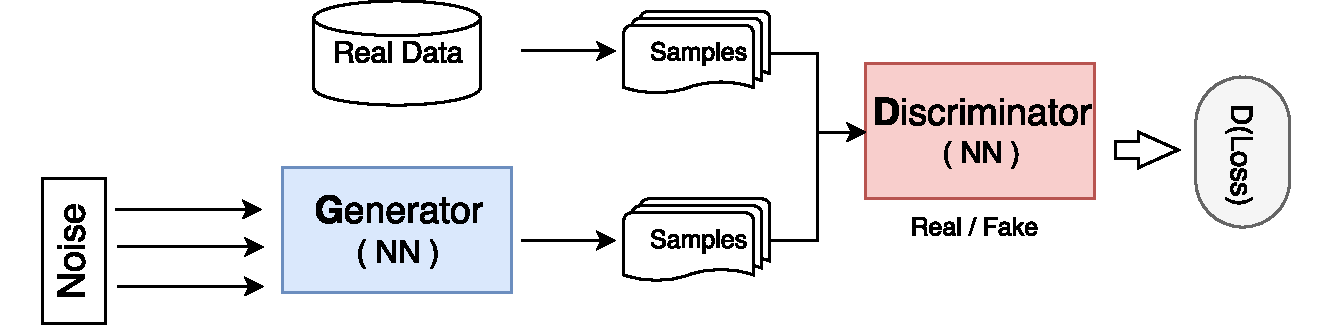
\includegraphics[width=0.6\textwidth]{GAN_basic}
			\caption{A strucutre of basic GANs} \label{fig:GAN-basic}
		\end{center}
	\end{figure}
	Figure 2 illustrates a basic structure of GANs. \textbf{G} generates fake data when arbitrary noise $z$ is given as an input through a NN composed of layers. Let $D(x)$ denote an output of \textbf{D} with $x$ as an input $x$. \textbf{D} is trained as $D(x)=1$ whenever $x$ is real otherwise $D(x)=0$. \textbf{G} tries to make $D(x) = 1$ for sample $x$ generated by \textbf{G}, and \textbf{D} tries to make $D(G(z)) = 0$ for any samples generated by $G(z)$, where $z$ is a randomly generated value. Therefore, the loss function $V(D,G)$ of GAN can be expressed as follows (ref.):
	\begin{align*}
	\min_G \max_D V(D,G)  = \mathbb{E}_{x:\text{real}}\left[\log D(x) \right]  + \mathbb{E}_{z:\text{randomly generated}} \left[\log(1-D(G(z))) \right] 
	\end{align*}
	Typical GANs have two NNs, which are trained iteratively. Each training iteration fixes either \textbf{G} or \textbf{D}, and updates the other un-fixed NN using well-known backpropagation algorithm. Contrary to ordinary DNNs that are good at classification of any given data, GANs are able to generate artificial data that look like real ones. GANs are actively studied and utilized for image-related applications especially with incorporating convolutional neural networks (CNN). There are little previous studies using GANs for solving combinatorial optimization problems (ref.). To the best of our knowledge, this study is the first attempt for solving the portfolio optimization problem using GANs. The basic idea is using the generating power of GANs to populate good candidates for the initial sets of assets to invest.
	
	\subsubsection{Generating Initial Sets of Assets using GAN}
	
	We use the GAN 's basic idea of learning networks with adversarial relationships between two networks to solve the problem of portfolio optimization. G determines the decision variable $w$ of the formulation, and D determines if the data generated from G is feasible. D is based on the formulation, and the sample data $G(z)$ generated checks both the feasibility of the solution and the quality of objective value. Specifically, when $ w_i $ is determined in G, the discriminator finds the sum of the objective value and the scaled value of the sum of values deviating from each constraint. Therefore, the value of loss in D is the sum of the degree of violation from the constraints and objective value. G is a deep NN structure consisting of one input layer, three hidden layers and one ouput layer. G tries to minimize the loss of D for the sample $G(z)$ generated from the random input noise $z \sim \mathcal {U}(-1,1)$. That is, the decision variable $ w $ generated in G is trained to be feasible for all constraints and the objective value to be minimized. Unlike the basic GAN structure, GAN for portfolio optimization has G for NN structure, but D is not, and only G is required to train. The loss function $V(G)$ of GAN can be expressed as follows :
	\begin{align*}
	\max_G \mathbb{E}_{x~p_{data}(x)}[\log(D(G(z)))] 
	\end{align*}
	The training is performed with a total of 2000 random datasets so that the loss value is minimized. At this time, the batch size is 1000 datasets, and then sample data is extracted after training 1000 datasets. At this time, if the value of D (G (z)) is larger than the threshold value (0.995) for sample data G (z), the solution is considered as feasible. 
	%Figure 3 shows the structure of G composed of NN and D composed of Formulation.
	In order to understand whether GAN is being well trained, we let GAN train with 2000 random datasets and examined the results. As a result of the experiments, we realized some of constraints are violate. However, we also realized that only about 5 percent of the constraints of the whole are violated, and the degree of violation is very small. Because of threshold, the results of trained GAN allow in some degree of infeasible. 
	
	
	%내용 추가 및 간단한 실험??????
	
	\begin{figure}[h] 
		\begin{center}
			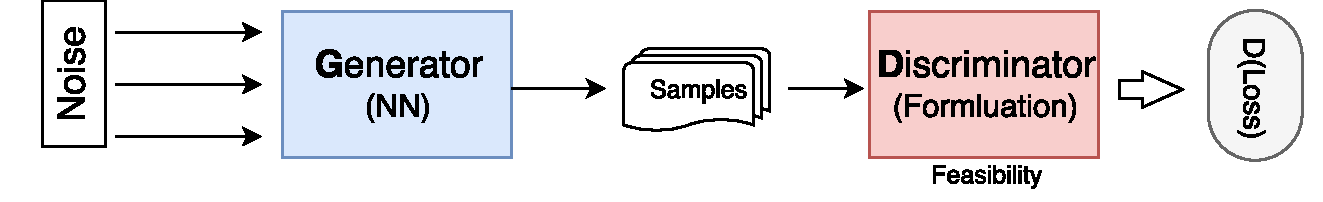
\includegraphics[width=0.6\textwidth]{GAN_port}
			\caption{The strucutre of GAN for portfolio optimization} \label{fig:GAN-port}
		\end{center}
	\end{figure}
	
	
	
	
	
	
	
	%Tracking Error가 왜 낮은지? obj val 을 낮추려 하니깐...!
	%According to Observation 2, Tracking Error should be raised. At this time, $d^T\Omega d$ can be expressed as $\quad w^T\Omega  w - w_{\text{bench}}^T\Omega  w_{\text{bench}} \quad$, which means that the difference between the benchmark weight and the portfolio weight is too small that Tracking Error does not satisfy the lower bound. In other words, the difference between the two weights must be increased to some extent to satisfy the constraints.
	
	
	%The bisectional search algorithm reflects that if some portfolio weights are increased, the othe portfolio weights of the assets become smaller because of the constraints(4). Since the following $  w_{\text{bench}}^T\Omega  w_{\text{bench}}  $ is fixed, it is required to satisfy the constraints by changing $w^T\Omega  w $. Because the weight value of all of the unselected assets from approximately 500 candidates is zero, the weight value is less than the benchmark weight value ($\because w_{bench} > 0$). On the other hand, the most of weight value of the 50 to 70 selected assets may be larger than the benchmark weights. Thus, we took a look for the average of portfolio weight and have noticed that about a third is smaller than average and two-thirds is larger than the average. Therefore, based on the average of portfolio weight, the portfolio weights are raised for the assets whose portfolio weight are larger than the average. Conversely, the assets whose portfolio weights are smaller than the average are decreased. As a result, the Tracking Error value becomes large, making the solution feasible.
	%	According to Observation 2, Tracking Error should be raised. For the given data, benchmark weights are distributed over about 500 assets, while the portfolio weight is 0 $(w_i = 0)$ for most of the remaining assets except for 50 to 70 selected assets. Thus, for non-selected assets $i$, $d_i$ can be expressed as $-w_{\text{bench}}$. In other words, if the assets whose $w_{\text{bench}}$ are large are not selected, the $\sum_{i \ inN}d_i$ becomes larger which means the Tracking Error is increased. %데이터특성상 bw가 작아서 이거로 키우는데는 무리가 있지 않을까 실질적으로 선택된 자산들을 조정하는게 효율적
	%	On the other hand, for the selected 50 to 70 assets, most $w_i $ are larger than $w_{\text{bench}}$. If the difference between $w_i$ and $w_{\text{bench}}$ is small, $ \sum_{i \ inN}d_i$  is also small. The difference between $w_{\text{bench}}$ and $w_i$ are required to be large for all selected assets,  so $ \sum_{i \ inN}d_i$ becomes larger when the difference between $w_{\text{bench}}$ and $w_i$ are large for all assets $i$. That is, the tracking error also becomes large. First, We took a look for the average of portfolio weight and have noticed that about two-thirds is smaller than average and a third is larger than the average. Therefore, based on the average of portfolio weight, the portfolio weights are raised for the assets whose portfolio weight are smaller than the average. Conversely, the assets whose portfolio weights are larger than the average are decreased. As a result, the Tracking Error value becomes large, making the solution feasible. To sum up, there are the ways to increase the tracking error by not selecting the assets with a larger $w_{\text{bench}}$ or by increasing the difference between $w_{\text{bench}}$ and $w_i$ for the selected assets. Since the value of the bench weight is practically insignificant, the method which increases the difference between $w_{\text{bench}}$ and $w_i$ for the selected assets is more efficient. 
	
	
	
	%The bisectional search algorithm reflects that if some portfolio weights are increased, the othe portfolio weights of the assets become smaller because of the constraints(4). Since the following $  w_{\text{bench}}^T\Omega  w_{\text{bench}}  $ is fixed, it is required to satisfy the constraints by changing $w^T\Omega  w $. Because the weight value of all of the unselected assets from approximately 500 candidates is zero, the weight value is less than the benchmark weight value ($\because w_{bench} > 0$). On the other hand, the most of weight value of the 50 to 70 selected assets may be larger than the benchmark weights. Thus, we took a look for the average of portfolio weight and have noticed that about a third is smaller than average and two-thirds is larger than the average. Therefore, based on the average of portfolio weight, the portfolio weights are raised for the assets whose portfolio weight are larger than the average. Conversely, the assets whose portfolio weights are smaller than the average are decreased. As a result, the Tracking Error value becomes large, making the solution feasible. 
	
	
	
	
	\underline{\textbf{Bisectional Search Algorithm}}:
	We applied the idea to the bisectional search algorithm. The bisectional search algorithm is an iterative algorithm that narrows the range and finds a feasible solution. When narrowing the range, if the feasible solution exists in the range, search in the right range based on the median of the range, and search in the left range if the feasible solution does not exist.	
	An example is shown in \ref{fig:bisection}. Let  $ \sum_{p\in P} w_p = 0.6$, where $P$ is a set of assets whose $w_i$ is smaller than the avarage of the portfolio weights. First, the solution is searched by dividing the interval between 0.8 and 1.0. If the solution is a feasible solution that satisfies both the range of Active Share and Tracking Error, narrow the range and search again in the left section. The search is stopped when the width of the range($\underline{Z} \sim \overline{Z}$) is less than the end condition which is set to 0.001. One of the feasible solutions, obtained from the bisectional search with the lowest objective value, is returned. Tracking Error increases as $\underline{Z}$ approaches to 1. Conversely, Tracking Error decreases as the $\overline{Z}$ approaches to $\sum_{p\in P}w_p$ (0.6 in the example). 
	\begin{figure}[h] 
		\begin{center}
			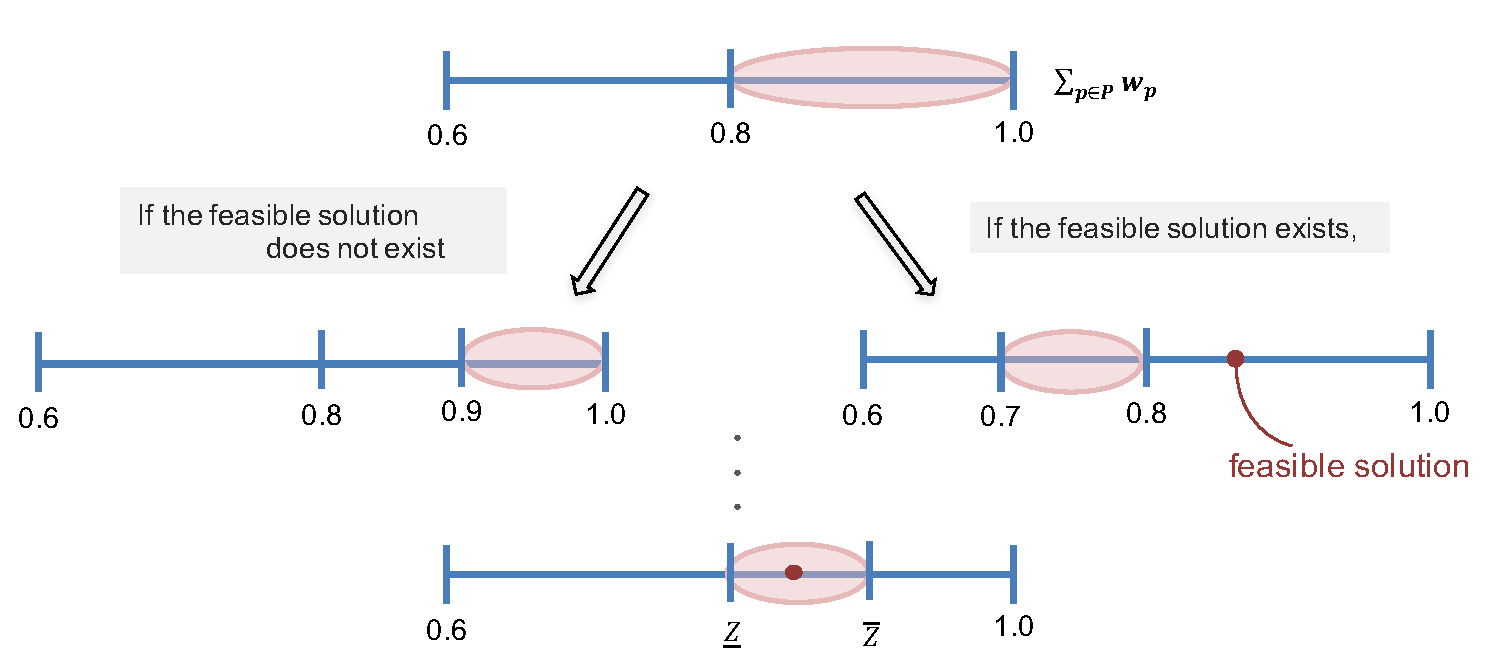
\includegraphics[width=0.75\textwidth]{bisection}
			\caption{An Example of Bisectional Search} \label{fig:bisection}
		\end{center}
	\end{figure}
	Therefore, the following constraints are derived through the bisectional algorithm : $\sum_{p \in P} w_i = (\underline{Z} +\overline{Z})/2 $ . Experimental results including the constraints show that Tracking Error is converged at the lower bound (0.05), except for the case where the difference between Tracking Error value and the lower bound is large before the start of the bisectional search.
	
	% bisectional algorithm 결론
	
	%\item[]\underline{Evolutionary Approach} : 
	
	% 진화 알고리즘 (ex.EDA)으로 접근. (간단한 실험?) -> 문제점 도출 : population의 수를 크게 두고 여러번 풀어 확률적 이론 등을 적용시키는 데에는 오랜시간 소요.
	
	
	
	
	\subsection{GAN-MP Hybrid Approach} %이름 
	We propose a new \textbf{GAN(Generative adversarial networks)-MP(Mathmatical Programming) Hybrid approach} that complements the disadvantages of formluation approach and neural network approach and enhances their advantages. Several limitations could be derived from the three approaches we present above. When solving the problem with the formulation appraoch, we could not find a reasonable solution because to consider about 500 assets per iteration the number of decision variables to decide and the number of constraints to be satisfied are too high . Especially, constraints (9) which select cardinalities considering the target range on number of stocks make the problem difficult. 
	In the case of Neural Network Approach, there is a great advantage in that a solution that does not get significantly out from the whole constraints and that has a good objective value can be considered at the same time. However, it is difficult to find a soluton satisfying the feasibility for all the constraints and the fact that the training time takes too much time. The GAN-MP hybrid approach is a highly efficient approach that maximizes the advantages of GAN and formulation-based optimizations. This appraoch consists of three steps as shown in Figure 4. Step1 is the process of finding the cardinality set which is the combination of the selected assets. The cardinality set selected in Step1 solves the QCQP problem with the selected assets fixed and finds the local optimal solution in Step2. According to the result of Step2, the update algorithm finds cardinality set that can reduce the objective value and improves the solution.
	\begin{figure}[h] 
		\begin{center}
			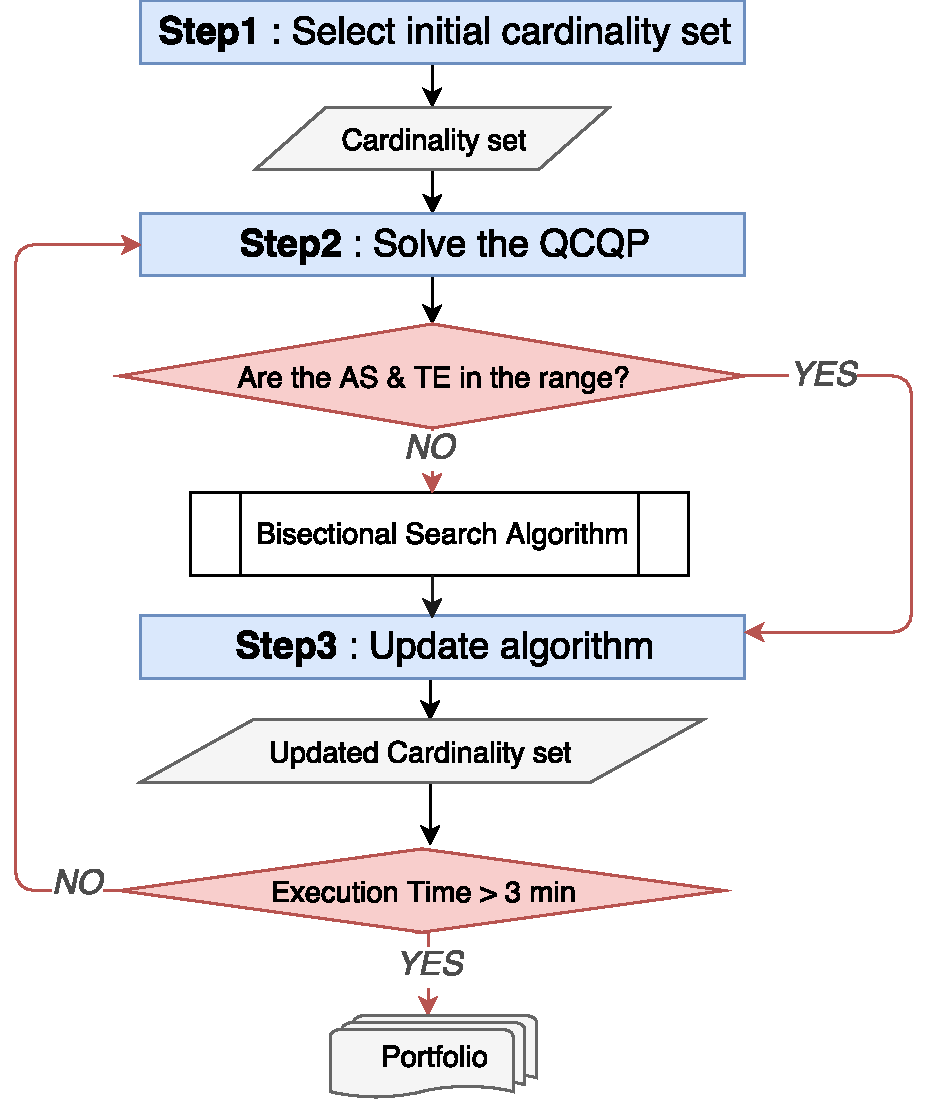
\includegraphics[width=0.45\textwidth]{flowchart}
			\caption{A Flowchart of Hybrid Approach} \label{fig:flowchart}
		\end{center}
	\end{figure}
	
	\underline{\textbf{(Step1) Select Initial Cardinality Set \& (Step2) Solve the QCQP }} :
	When the number of assets to be considered is large, the problem becomes large as the number of constraints increases as well as decision variables. 
	Thus, the process of step1 filters out good assets that are crucial for minimizing the objective value. At this time, the set of good assets must meet the following criteria.
	\begin{itemize}
		\item[]\textbf{Criterion 1.} The combination of assets should be satisfy all constraints
		\item[]\textbf{Criterion 2.} The combination of assets is chosen to minimize the risk and maximize return.
	\end{itemize}
	In order to meet these criteria , the whole assets are required to be considered. We propose a formulation approach that finds the solution through Mixed Integer Programming (MIP) and a neural network-based GAN as a way to satisfy constraints and to take low values of objective value globally. Therefore, the experiments are carried out with two algorithms (MIP, GAN). For a given time, the MIP proceeds branch and bound(B\&B) and the GAN proceeds to train the generator consisting of NN (Step1). After the given time, the assets, $w_i> 0.001$ for all asset $i \in N$ ,were extracted in the best solution found in each algorithm. The portfolio optimization problem that determines the weight of each assets as the cardinality set is fixed (Step2) . Accordingly, constraints (9) does not to be considered anymore, and the set $N$ changes to $S$, which stands for set of selected assets for all of the constraints. Therefore, the number of constraints and decision varaibles are reduced. 
	% The following experiments were conducted to evaluate the performance of the algorithms.
	\begin{itemize}
		\item Experiment Environment
		\begin{itemize}
			\item Number of Experiments : 50 times
			\item The B\&B Timelimit for MIP : 90 seconds  \begin{scriptsize}	(minimun time for feasible solution)	\end{scriptsize}
			\item Training Time for GAN : 20 seconds
			\item Solver of MIP : Cplex
			\item Deep Learning Library : Pytorch
			\item Data of the first period (2007/01/03)
		\end{itemize}
		\item Experiment Results :
		\begin{figure}[h]
			\begin{center}
				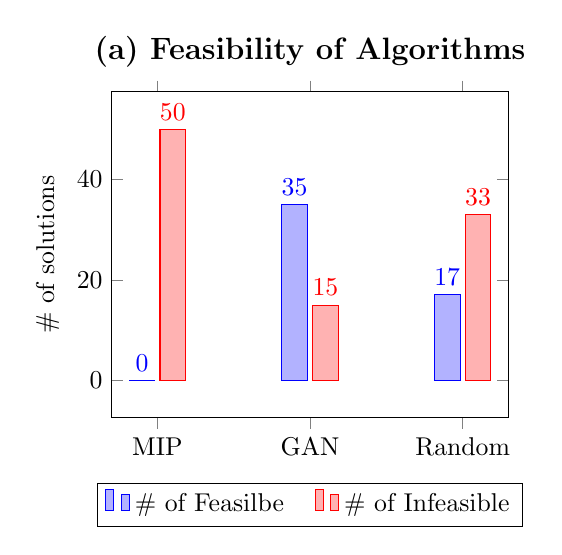
\begin{tikzpicture}[scale=0.93]
				\begin{axis}[
				ybar,
				enlargelimits=0.15,
				legend style={at={(0.5,-0.20)},
					anchor=north,legend columns=-1},
				ylabel={\# of solutions},
				symbolic x coords={MIP,GAN, Random},
				xtick=data,
				nodes near coords,
				nodes near coords align={vertical},
				title={\large\textbf{(a) Feasibility of Algorithms}}
				]
				\addplot coordinates {(MIP,0) (GAN,35) (Random,17)};
				\addplot coordinates {(MIP,50) (GAN,15) (Random,33)};
				\legend{\# of Feasilbe$\quad$, \# of Infeasible}
				
				\end{axis}
				\end{tikzpicture} 
				\quad
				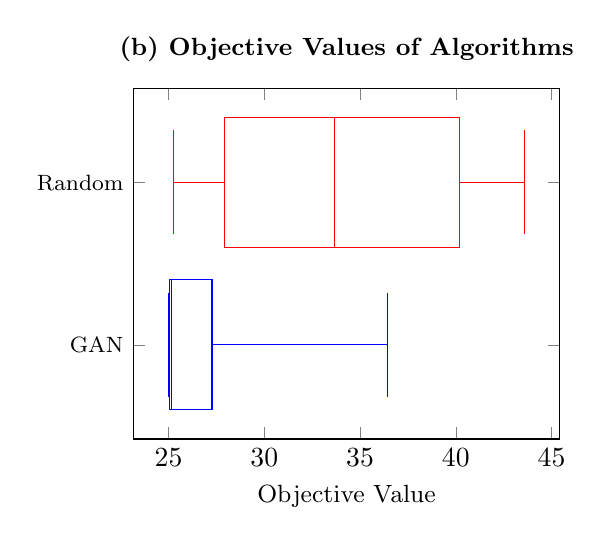
\begin{tikzpicture}[scale=1.]
				\begin{axis}
				[
				ytick={1,2},
				yticklabels={\footnotesize GAN, \footnotesize Random},
				xlabel={\small Objective Value  },
				title={\small\textbf{(b) Objective Values of Algorithms}}
				]
				\addplot+[
				boxplot prepared={
					median=25.14,
					upper quartile= 27.27,
					lower quartile=25.056,
					upper whisker=36.43,
					lower whisker=25.013
				},
				] coordinates {};
				\addplot+[
				boxplot prepared={
					median=33.66,
					upper quartile=40.18,
					lower quartile=27.90,
					upper whisker=43.58,
					lower whisker=25.26
				},
				] coordinates {};
				
				\end{axis}
				\end{tikzpicture}
				\caption{Results of Algorithms} \label{fig:feasi}
			\end{center}
		\end{figure}
		\item[]  The cardinality sets are derived by solving MIP problem with the Cplex, and  all of the results were infeasible when solving the portfolio optimization problem with the fixed assets. One reason that cannot derive the feasible solutions is that Tracking Error is too low because the constraints of Tracking Error are not reflected in MIP. Thus, Cplex does not suit for selecting initial cardinality set.  If random samples are specified as an initial cardinality set, the solutions are often infeasible, and objective values are lower than GAN. \underline{Therefore, the initial cardinality set is assigned to the GAN} because the feasible solution is derived more reliably than others, and the objective value is relatively low. 
		
		\item Threshold and Suggestion :
		
		GAN is composed of NNs, and the result quality and training time vary depending on computing environment of NN. Therefore, we recommend that Principal could improve the training speed and quality by using GPU-accelerated computing or through some advanced technologies such as Amazon Cloud services. By improving the environment, more accurate and better solutions are derived by adjusting the hidden layer addition and the learning rate that we could not reflect now because of computing power. 
		
	\end{itemize}
	
	
	
	\begin{figure}[h] 
		\begin{center}
			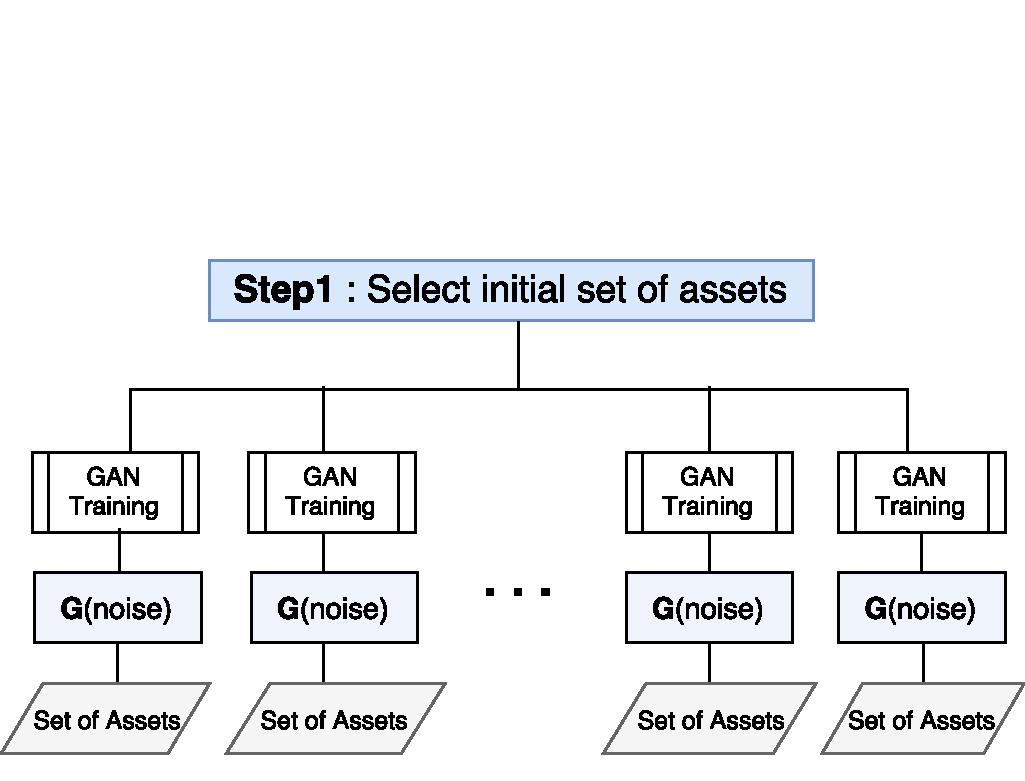
\includegraphics[width=0.6\textwidth]{step1}
			\caption{A Flowchart of Hybrid Approach} \label{fig:step1}
		\end{center}
	\end{figure}
	
	
	We present a model that can maximize the benefits of GAN in a given situation. The major advantage of the GAN is that it can extract solutions whenever noises are given to G by learning the weight and bias of the generator.
	The server that currently runs the code has eight cores, so we figure out the server can run up to 8 GANs simultaneously on 8 cores. Therefore, we use the parallel process to be 8 GANs training at the same time and then obtain 8 initial cardinality sets each as a result. The parallel process uses the Python Library of Ipython Parallel (https://ipyparallel.readthedocs.io), and Figure 6 shows the process of obtaining 8 sets of cardinality sets by running 8 GANs using Ipython Parallel.
	
	\underline{\textbf{(Step3) Update Algorithm }} :  The assets to be included in the portfolio are selected by GAN, and the MIP is solved by Cplex for determining weights to each assets. 
	As a result of solving QCQP problems, the solutions are derived. At this time, the local optimal solution may be improved depending on which asset is selected. Therefore, based on good initial cardinality set, it is necessary to perform a local search by changing the items of the asset, the weight of the asset, and the number of selected assets. However, if the initial cardinality set obtained from the GAN is not good in Step 1, changing the number of assets does not improve the result significantly. To determine the bad cardinality set, we check the quality of the solution when we solve the MIP with the initial cardinality set before updating the cardinality set. The following process is performed according to the result of 8 solutions. For 4 cardinality sets with bad results, it is required to find a new initial cardinality set ($\rightarrow$ Step1. Select Initial Cardinality Set). For 4 the other cardinality sets with good results, it adjusts the assets to improve results ($\rightarrow$ Step3. Update Algorithm). 
	
	%Update Algorithm
	
	\begin{figure}[h] 
		\begin{center}
			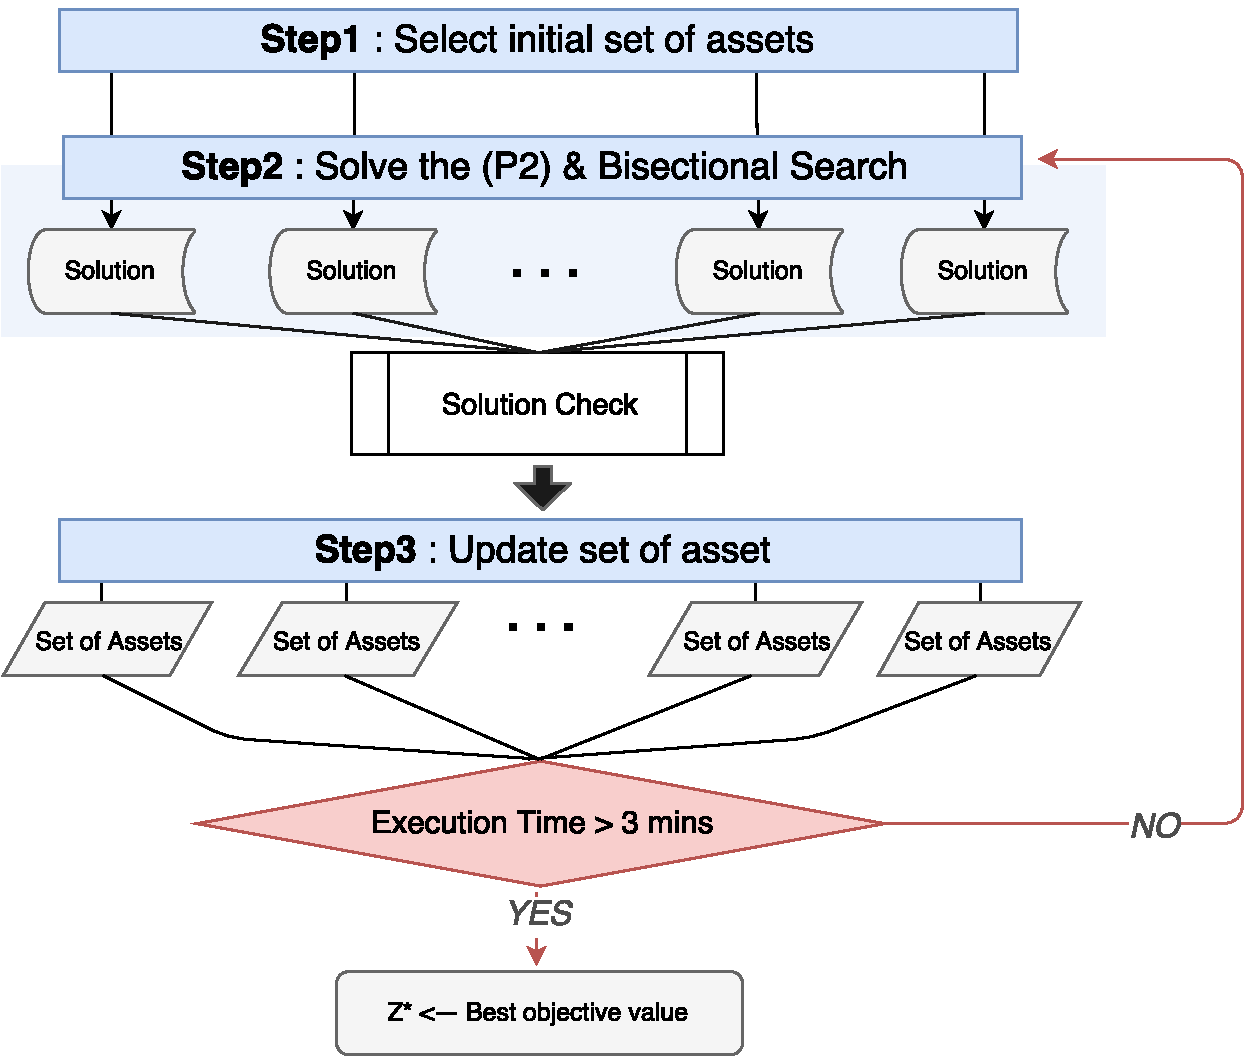
\includegraphics[width=0.65\textwidth]{step3}
			\caption{A Flowchart of Hybrid Approach} \label{fig:step3}
		\end{center}
	\end{figure}
	
	
	Basically, update algorithm has 2 goals. 
	\begin{itemize}
		\item[(1)] One is that the update algorithm finds one or multiple assets whose objective value is lower when one or multiple assets is/are added or removed. 
		\item[(2)] The other is if the result of current cardinality set is infeasible, it also adjusts the cardinality set so that it becomes feasible.
	\end{itemize}
	To accomplish these two goals, the update aglrithm is supposed to adjust the cardinality set solving the problem and improving the solution until it is reachead to the end condition. First, the update algorithm finds out which asset gets better to lower the objective value when it gets out of the portfolio, and which asset should be added to improve the outcome. From the viewpoint of determining which asset is included in the portfolio, there is a great difficulty in deriving an objective value that can be obtained only when the weight of each asset is determined. We therefore take into account the maximum value that an asset has on the determination of the objective value. In the objective function, the risk is minimized while the return is maximized. Let $C$ is a set of assets whose asset $i$ is in cardinality set, and $K$ is a set of assets whose asset is not in cardinality set, that is candidate set for update algorithm. In order to find an good asset with higher return and lower risk, return and risk for the candidate asset $k \in K$ are calculated as follows:
	\begin{itemize}
		\item[\textbullet] Return = The maximum return that occurs as the asset $k$ comes in $\Rightarrow \alpha_k$
		\item[\textbullet] Risk = The maximum risk that occurs as the asset $k$ comes in $\Rightarrow \sum_{c \in C}\Omega_{ck} + \Omega_{kk}$
	\end{itemize}
	On the contrary, the asset $c$\textasciiacute$\,$ that increases the objective value because the risk is large and the return is small among the assets included in the current cardinality set is also determined by the following criteria : 
	\begin{itemize}
		\item[\textbullet] Return = The maximum return that decreases as the asset $c$\textasciiacute$\,$ leaves the cardinality set $\Rightarrow \alpha_{{c}'}$
		\item[\textbullet] Risk =  The maximum risk that decreases as the asset $c$\textasciiacute$\,$ leaves the cardinality set $\Rightarrow \sum_{c \in \{c | c \in C \, \text{and} \, c \neq \ {c}' \}}\Omega_{c {c}'} + \Omega_{{c}' {c}'}$
	\end{itemize}
	Therefore, in order to improve the objective function, the update algorithm minimizes the Risk $-$ Return for the new candidate asset $k$ and eliminates the asset $c$\textasciiacute$\,$ which have a bad effect on the existing cardinality set. Repeating this process can result in a local optimal solution as a result of obtaining a good cardinality set. However, infeasible cardinality sets can be obtained in many cases when considering the risk and return to obtain a good cardinality set. The cardinality set is infeasible, which means that when a QCQP problem is solved after fixing an asset with a cardinality set, a feasible solution can not be found in violation of some constraints. We have noticed that most infeasilbe cardinality sets occur in Constraints 7 and 8 indicating the limits of Sector Active Share and Market Cap Quintile (MCAPQ) Active Share.
	To see why, we took a look at data for the first date (date of January 3rd, 2007 ) of a given dataset. Figure 6 shows the sum of the weights for each sector and MCㅁAPQ to satisfy Constraints 6 and 7. Because $w_\text{bench} $ is different for each asset, the scope varies depending on what asset is included in the sector and the MCPQA. In other words, when the sum of each sector and MCAPQ is sensitive, it becomes a difficult constraint to satisfy. Therefore, if the constraints 6 and 7 are violated in the process of improving the cardinality set, adding deficient sector and mcapq assets is prevent infeasible. 
	\begin{figure}[h]
		\begin{center}
			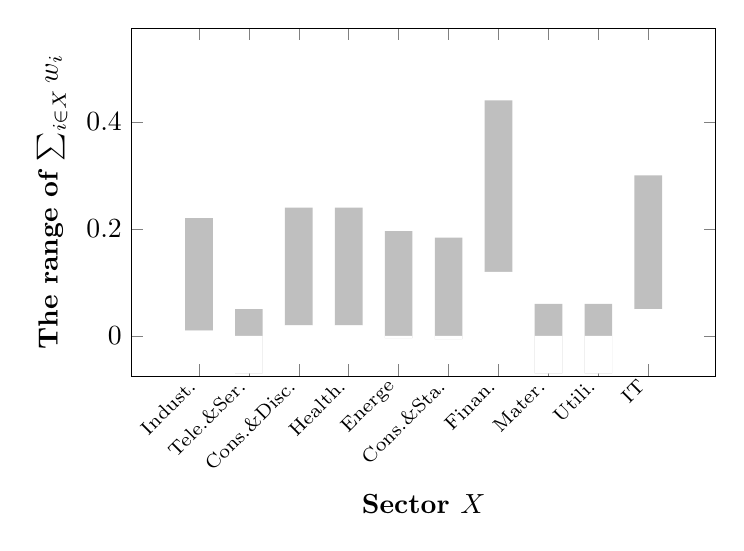
\begin{tikzpicture}
			\begin{axis}[
			width=9cm,
			height=6cm,
			ybar stacked,
			bar width=10pt,
			enlargelimits=0.15,
			legend style={at={(0.5,-1)},
				anchor=north,legend columns=-1},
			ylabel={\textbf{The range of $\sum_{i \in X}w_i$}},
			xlabel={\textbf{Sector $X$}},
			xlabel near ticks,
			ymin=0,
			ymax=0.5,
			symbolic x coords={Indust., Tele.\&Ser., Cons.\&Disc., Health., 
				Energe, Cons.\&Sta., Finan.,Mater.,Utili.,IT},
			xtick=data,
			x tick label style={rotate=45,anchor=east},
			xticklabel style = {font=\scriptsize}
			]
			
			\addplot+[ybar,color=black,draw=none,fill=white ] plot coordinates {(Indust., 0.01)
				(Tele.\&Ser., -0.07)
				(Cons.\&Disc., 0.02)
				(Health., 0.02)
				(Energe, -0.004)
				(Cons.\&Sta., -0.006)
				(Finan., 0.12)
				(Mater., -0.07)
				(Utili., -0.07)
				(IT, 0.05)
			};
			\addplot+[ybar,color=black, draw=none,fill=lightgray] plot coordinates { (Indust., 0.21)
				(Tele.\&Ser., 0.12)
				(Cons.\&Disc., 0.22)
				(Health., 0.22)
				(Energe, 0.2)
				(Cons.\&Sta., 0.19)
				(Finan., 0.32)
				(Mater., 0.13)
				(Utili., 0.13)
				(IT, 0.25)
			};
			
			\end{axis}
			\end{tikzpicture}
			\quad
			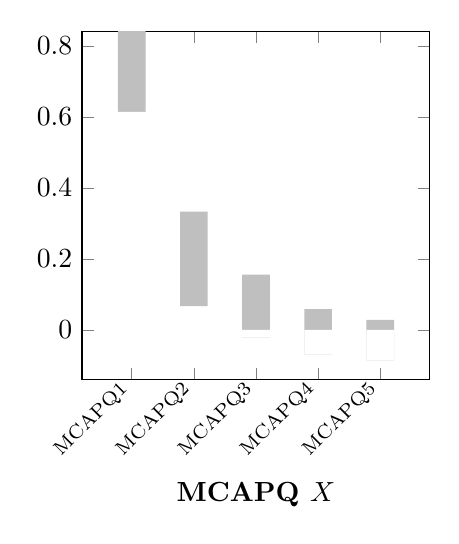
\begin{tikzpicture}
			\begin{axis}[
			width=6cm,
			height=6cm,
			ybar stacked,
			bar width=10pt,
			enlargelimits=0.2,
			legend style={at={(0.5,-1)},
				anchor=north,legend columns=-1},
			xlabel={\textbf{MCAPQ $X$}},
			xlabel near ticks,
			ymin=0,
			ymax=0.7,
			symbolic x coords={MCAPQ1, MCAPQ2, MCAPQ3, MCAPQ4, MCAPQ5},
			xtick=data,
			xticklabel style = {font=\scriptsize},
			x tick label style={rotate=45,anchor=east},
			]
			\addplot+[ybar,color=black,draw=none,fill=white ] plot coordinates {(MCAPQ1, 0.613783144)
				(MCAPQ2, 0.066327628)
				(MCAPQ3, -0.022)
				(MCAPQ4, -0.07)
				(MCAPQ5, -0.086)};
			\addplot+[ybar,color=black, draw=none,fill=lightgray] plot coordinates { (MCAPQ1, 0.81378314399999996)
				(MCAPQ2, 0.26632762799999998)
				(MCAPQ3, 0.17779934600000002)
				(MCAPQ4, 0.12814390000000001)
				(MCAPQ5, 0.113946004)	};
			\end{axis}
			\end{tikzpicture}
			\caption{The sum of the weights for each Sector and MCAPQ}
		\end{center}
	\end{figure}
	
	
	
	
	\section*{Analytics Solution and Results}
	\setcounter{subsection}{0}
	
	In this section, we report results of computational experiments for solving portfolio optimization with the methodology we present. First, we show how to set the parameter $\lambda$ to be considered in the problem in order to obtain the optimal solution before proceeding with the experiment. Also, we present how rebalancing reflects in our proposed model. Finally, the results of the computational experiments with the determined parameters are present.
	
	\subsection{Parameter Setting}
	
	To set parameters, various experimental analyzes are required with real data. However, there is a limit to obtaining the real data such as $\alpha, \Omega, \beta$, and bench weight from the historical data. we assume that the year 2007 is a parameter adjustment period, and analyzed the data in 2007. 
	
	\underline{\textbf{The Parameter $\lambda$}}: Parameter $ \lambda $ reflects how much return will be considered relative to risk in objective function. When the value of $ \lambda $ is large, the return is considered a lot, and when the $ \lambda $ value is low, the risk is considered more. We used 2007 data to analyze whether the $d^{T} \alpha$, which represents a return on objective, has an influence on the overall return index ($r_{opt}$) as we adjusted the $\lambda$. In other words, as the lambda value increases, more revenue will be taken into account, so that it can be inferred that the $r_{opt}$  is more affected by return or risk.
	%실험 
	%실험결과: 어떤 지표와도 상관이 없다.
	%원인 1) risk 와 return의 범위 : 25언저리 vs 0.5 (람다가10일때) 
	%		2) 실제 return과 r_opt와의 관계가 없었음
	%결론 : 큰 차이가 없으므로 default 값인 1을 사용
	
	\subsection{Rabalancing}
	
	Portfolio turnover depends on how many assets in the portfolio chance from rebalance to rebalance, and the value of turnover has effects on Information Ratio(IR). Therefore, it is required to consider turnover in the portfolio optimization. We apply turnover to the both GAN for finding initial cardinality set and QCQP problem for determining the weight of the selected asset. For applying it to GAN, the calculated $\text{turnover}_{t} (\sum_{i \ inN}|w_{i,t}-w_{i,t-1}^{pre}|)$was directly taken into account in the objective function. On the other hand,for applying it to MIP, it should be linearlized. We reflect turnover into the objective function in MIP as follows: 
	\begin{align*}
	\text{(MIP)} \quad \min \quad & d^T\Omega d  -  \lambda d^{T}\alpha - \omega \sum_{i \in N}o_i \quad  \quad \quad\text{(2*)}\\
	\text{s.t } \quad & (3) - (11)\\
	& o_i \geq w_{i,t}-w_{i,t-1}^{pre}, \quad \forall{i \in N} \\
	& o_i \geq -w_{i,t}+w_{i,t-1}^{pre}, \quad \forall{i \in N} 
	\end{align*}
	The decision variables $o_i$ is the difference between $w_i$ of previous period(t-1) and $w_i$ of current(t) period for all asset $i \in N$. Because of constraints added, $ w_{i,t}-w_{i,t-1}^{pre}$ is positive for all asset $i \in N$. The parameter $\omega$ represents the weight of turnover for objective value considering risk and return. 
	
	\underline{\textbf{The Parameter $ \omega$}}: 
	%실험내용
	%실험결과 및 결론
	
	\subsection{Computational Experiments}
	
	\underline{\textbf{Experiment environment}} : The experiments were performed on an Intel Core 3.5 GHz PC with 32GB memory and ILOG CPLEX 12.6 were used as an MIP solver, and Pytorch for Python 3.6 was used as a deep learning framework. 
	
	
	\underline{\textbf{The Portfolio Performance Statistics}} : 
	\begin{center}
		\textbf{Portfolio Performance Statistics}\vspace*{-14pt}
	\end{center}
	
	\begin{table}[htbp]
		\def\arraystretch{1.4}
		\begin{center}
			\begin{tabular}{|l|c|c|}
				\hline
				\textbf{2007-01-01 to 2016-12-31}& 
				\textbf{Portfolio}& 
				\textbf{Benchmark} \\
				\hline
				Cumulative Return& 
				{\%}& 
				{\%} \\
				\hline
				Annualized Return& 
				{\%}& 
				{\%} \\
				\hline
				Annualized Excess Return& 
				{\%}& 
				-- \\
				\hline
				Annualized Tracking Error& 
				{\%}& 
				-- \\
				\hline
				Sharpe Ratio& 
				& 
				\\
				\hline
				Information Ratio& 
				& 
				-- \\
				\hline
			\end{tabular}
			\label{tab1}
		\end{center}
	\end{table}
	
	
	\subsection{Dealing Uncertainty of $\alpha$} 
	
	The results obtained earlier are derived by deterministic values which are $\alpha$ and $\Omega$. However, this is a parameter value with uncertainty, so we figure out the change of $\alpha$ and $\Omega$ in the historical data.  We first tried to secure the value of risk and alpha score for 2007 by analyzing the historical data. The analyzed data is obtained from Yahoo Finance and is historical data from 1970 to 2017. For the first time, we are looking at the risk of an asset in 2006 with extensive historical data. We obtained data on close stock prices for approximately 400 assets from historical data among 492 assets included in January 3, 2007 in S \& P 500 and derived a cross covariance matrix. And then, the correlation between the covariance matrix and the full matrix of $\Omega$ was derived. We expected a large correlation between the two matrices, but the result was not. It is judged that it is difficult to deduce $\Omega$ value from the covariance matrix derived from historical data. Therefore, we obtain the range of parameter change for each asset with the first year data received from the Principal and reflect it in the following robust optimization. %왜 \alpha만 고려하는가? 쉽게 고려할 수 있는 부분?
	
	Let set $U := \{ \tilde \alpha \in \mathbb{R}^{|N|}  \mid \tilde \alpha_i = \alpha_i + \bar{\alpha}_i \gamma_i , \quad -1 \leq \gamma_i\leq 1 , \quad \sum_{i} |\gamma_i| = \Gamma \}$, which contains all possible realizations of $\alpha$. Our goal is to consider the worst-case realization of $U$, which means that the expected return of the active weight ($d^T \tilde{\alpha}$) is guaranteed above the worst-case value. The mathematical formulation addressing the uncertainty of $\alpha$ is stated as follows:
	\begin{align}
	\text{(RP)} \quad \min~ & d^T \Omega d - \lambda \min_{\tilde{\alpha} \in U} \{d^T \tilde{\alpha} \} \label{eq:RP:obj}\\
	\text{s.t. } 
	& \eqref{eq:P:activeweight}, \eqref{eq:P:nonn} - \eqref{eq:P:TE}. \notag
	\end{align}
	For a given $d$, the inner minimization problem is stated as
	\begin{align}
	\min_{\tilde{\alpha} \in U} \{ d^T \tilde{\alpha} \} &= \min \left\{ \sum_{i \in N} d_i (\alpha_i + \bar{\alpha}_i \gamma_i ) : -1 \le \gamma_i \le 1, \forall i \in N, \sum_{i \in N} |\gamma_i| = \Gamma  \right\}\\
	&= d^T \alpha - \max \left\{ \sum_{i \in N} |d_i| \bar{\alpha}_i \gamma_i : 0 \le \gamma_i \le 1, \forall i \in N, \sum_{i \in N} \gamma_i = \Gamma  \right\}.
	\end{align}
	As shown by \cite{bertsimas2004price}, the latter maximization problem has an integral polyhedron. Using the linear programming duality theory, it is easily shown that the following holds:
	\begin{align}
	&\max \left\{ \sum_{i \in N} |d_i| \bar{\alpha}_i \gamma_i : 0 \le \gamma_i \le 1, \forall i \in N, \sum_{i \in N} \gamma_i = \Gamma  \right\} =\\
	&\min \left\{ \Gamma \pi + \sum_{i \in N} \theta_i : \pi + \theta_i \ge \bar{a}_i p_i,~ -p_i \le d_i \le p_i,~ \theta_i \ge 0, ~\forall i \in N   \right\}
	\end{align}
	Then, the problem (RP) can be reformulated as
	\begin{align}
	\text{(RP1)} \quad \min~ & d^T \Omega d - \lambda \left[ d^T \alpha - \left(\Gamma \pi + \sum_{i \in N} \theta_i \right) \right] \label{eq:RP1:obj}\\
	\text{s.t. } 
	& \eqref{eq:P:activeweight}, \eqref{eq:P:nonn} - \eqref{eq:P:TE}, \notag\\
	& \pi + \theta_i \ge \bar{\alpha}_i p_i, & \forall i \in N, \\
	& -p_i \le d_i \le p_i, & \forall i \in N,\\
	& \theta_i \ge 0, & \forall i \in N.
	\end{align}
	Note that (RP1) reduces to the problem (P) when $\Gamma=0$. Because reformulation of (RP1) involves only linear constraints and continuous decision variables, the proposed algorithm for (P) can be used for solving (RP1) without further modifications except the mathematical formulation. 
	
	
	
	
	\section*{References}
	
	\bgroup
	\parskip0pt
	
	Please follow guidelines in the \textit{Chicago Manual of Style,} 16$^{\text{th}}$ Edition. Here are examples: 
	
	\begin{itemize}
		\item[--] Journal article: Flynn J, Gartska SK (1990) A dynamic inventory model with periodic auditing. \textit{Oper. Res.} 38(6):1089--1103. 
		\item[--] Book: Makridakis S, Wheelwright SC, McGee VE (1983) \textit{Forecasting: Methods and Applications}, 2nd ed. (John Wiley {\&} Sons, New York). 
		\item[--] Edited Book: Martello S, Toth P (1979) The 0-1 knapsack problem. Christofides N, Mingozzi A, Sandi C, eds. \textit{Combinatorial Optimization} (John Wiley {\&} Sons, New York), 237--279.
		\item[--] Online reference, fictional example: American Mathematical Institute (2005) Better predictors of geospatial variability. Retrieved June 14, 2005, \underline {www.mathematicsinstitute}.
		
		
	\end{itemize}
	
	
	\bibliographystyle{chicago}
	\bibliography{informs}
	
	\egroup
	
\end{document}